
The past experiments were all regarding \textit{readout calibration}, from those we extracted the main parameters required for measurements:
\begin{itemize}
    \item waiting time for acquisition (\textit{time of flight});
    \item frequency of the readout pulse (so of the resonator);
    \item amplitude of the readout pulse;
    \item estimation of ground state;
    \item estimation of the \textit{sweetspot}. For flux tunable systems every experiment will be conducted at the sweetspot unless otherwise stated.
\end{itemize}
With these components we can proceed to look directly for the qubit that for now we saw only indirectly with the \textit{punchout} experiment (and in flux resonator spectroscopy).

If the resonator spectroscopy experiments is a \textit{single-tone spectroscopy}, to find the qubit frequency we need a \textit{two-tone spectroscopy}.
The idea is to send a first tone through the qubit drive line and then execute a measurement (so a second tone). 
The first tone will be changed in frequency and won't have any effect on the qubit state unless the frequency matches the qubit transition one.
Looking at \cref{eq:probability_1} we will have $\Delta_d^2\gg A \rightarrow P_1(t) = 0$.\\
However, if the drive frequency is "near" the resonant qubit frequency, the qubit will get excited, thus changing the amplitude of the acquired signal.

The qubit spectroscopy experiment~\cite{Schuster2005, Schuster2007} is very similar to the resonator one: we fire a drive pulse at a certain frequency; \textit{after} it, we perform a measurement, we wait for the qubit to relax, we repeat the experiment at different frequencies and then plot drive frequency vs measured amplitude, looking for a Lorentzian (downward if the resonator was upward and vice versa) as in \cref{fig:qubit_spectroscopy_sketch}.

\begin{figure}[ht]
    \centering
    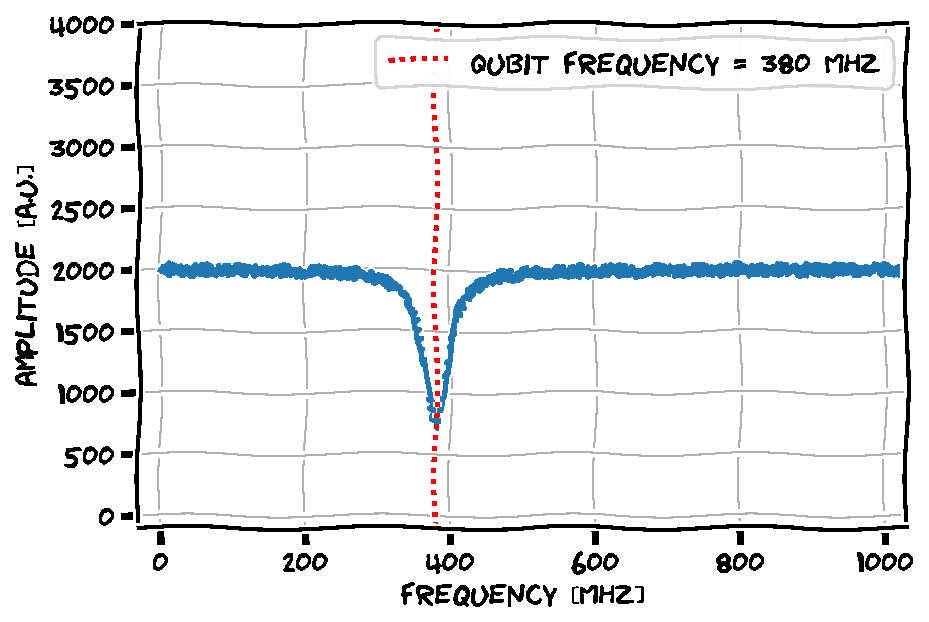
\includegraphics[width=8cm]{characterization/figures/qubit_spectroscopy_sketch.pdf}
    \caption{Sketch of the plot expected for a qubit spectroscopy experiment.}
    \label{fig:qubit_spectroscopy_sketch}
\end{figure}

As always there are several variables and phenomena to take into account:
\begin{itemize}
    \item the drive pulse will be, at the end of the calibration, a DRAG pulse with a length of $\approx 40$ ns, but here we are interested in calibrating only the frequency: therefore we use rectangular pulses with length of $1-2$ $\mu$s;
    \item it is important to wait for the drive pulse to end so that we avoid the \textit{Stark effect/shift}~\cite{Schuster2005}, but we should not wait any time more than strictly necessary. Because of that it is important to have all the cables of the same length;
    \item if we send too much power we could end up exciting the qubit even at "wrong" frequencies. We can check this by looking at the average amplitude measured: if it is not at the same level of what we defined in the resonator spectroscopy experiments as the ground state, than we are probably always exciting the qubit and we should reduce the amplitude of the drive. At the same time if we do not see any excitation we could need to increase the amplitude;
    \item having a large relaxation time is not strictly needed, in the sense that we could even initially perform this experiment without waiting for relaxations. However this will lead to not exact results and to an asymmetric Lorentzian: in fact we will excite the qubit with frequency A, measure the excited state, then apply frequency B that wouldn't excite the qubit, but still measure the excited state. Anyway, having a way of executing a fast version of the experiment may still be useful;
    \item the frequency step of the scan is clearly very important. A step of $100$ MHz should be enough fine;
    \item it is important to be aware of potential aliasing phenomena and signal images caused by local oscillators or DDS. For every found peak/deep, always ask yourself if it can be caused by these phenomena and, eventually, exclude it using the proper filters.
\end{itemize}

Without knowing anything about the qubit frequency, this experiment is not particularly easy: it can happen that the scan is at the right frequencies, but that there is no excitation for different reasons (for example the drive pulse has not enough amplitude).
Or that we focus on the wrong frequencies because in some scans there seem to be a peak (maybe because of aliasing or jsut noise).

In \cref{fig:qubit_spectroscopy_aliased} we can see a first, fairly unfortunate, qubit spectroscopy done for a single qubit chip with the \RFSoC.
See that the S/N ratio is not good at all, the peaks are very asymmetric (since the relaxation time was set to 0) and, clearly, there are two peaks for what should be a single qubit.\\
Multiple peaks can be caused by different phenomena, but here it is easy to see that the two peaks are equally distant (and opposite) from $f_s/2$ (half of the DAC sampling frequency) so we are actually seeing the effect of aliasing (as described in \cref{sec:aliasing}).
\begin{figure}[ht]
    \makebox[\textwidth][c]{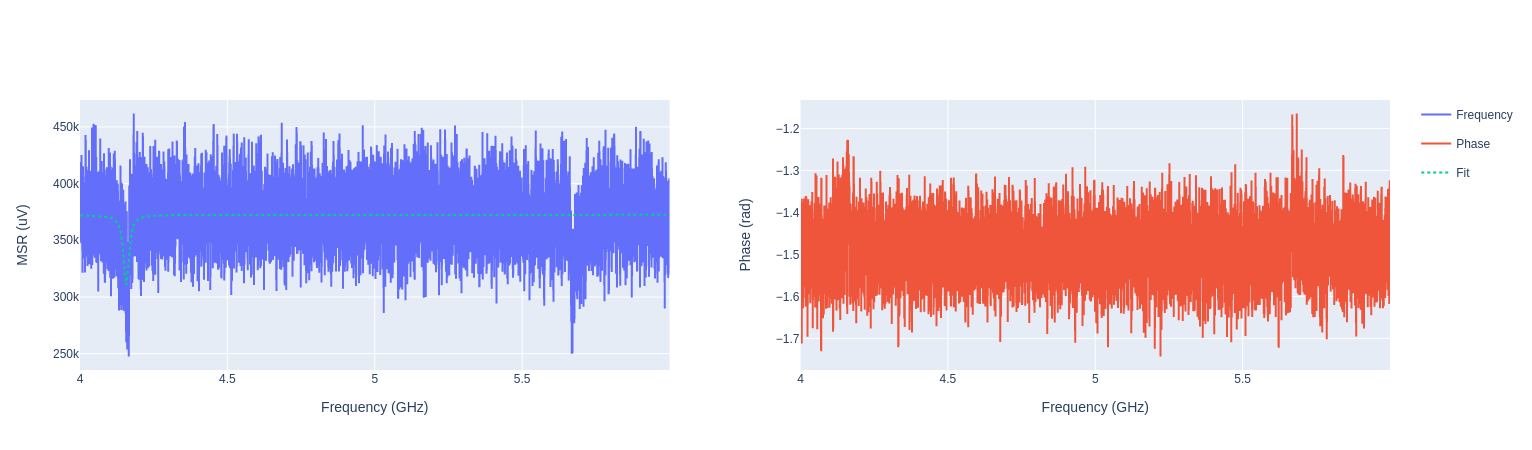
\includegraphics[width=1.3\textwidth]{characterization/figures/qubit_spectroscopy_aliased.png}}
    \caption{Example of a qubit spectroscopy experiment with clear aliasing.}
    \label{fig:qubit_spectroscopy_aliased}
\end{figure}
To check which one of the two peaks is the correct one, to properly characterize the qubit, the experimenter can add a frequency filter to remove one of the two peak: if it does not disappear, it is the image.
\\
Usually, anyway, just a single peak will be present, as in \cref{fig:qubit_spectroscopy}.

\begin{figure}[ht]
    \makebox[\textwidth][c]{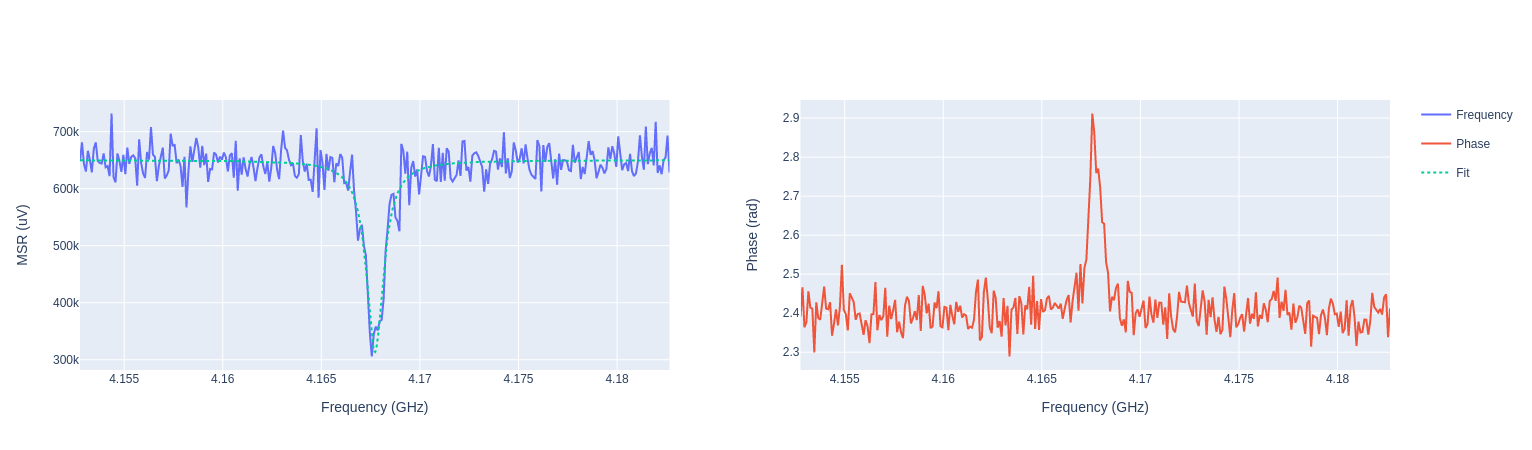
\includegraphics[width=1.3\textwidth]{characterization/figures/qubit_spectroscopy.png}}
    \caption{Example of a qubit spectroscopy experiment.}
    \label{fig:qubit_spectroscopy}
\end{figure}
Note that now, having both the qubit frequency and the resonator frequency for high e low power, we can also get the value of the coupling factor from the dispersive shift relation:
\begin{equation}
    \omega_{rh} - \omega_{rl} = \chi = \frac{g^2}{\Delta} = \frac{g^2}{\omega_{rl} - \omega_q} \rightarrow g =  \sqrt{(\omega_{rl} - \omega_q)(\omega_{rh} - \omega_{rl})}
\end{equation}

\begin{figure}[ht]
    \makebox[\textwidth][c]{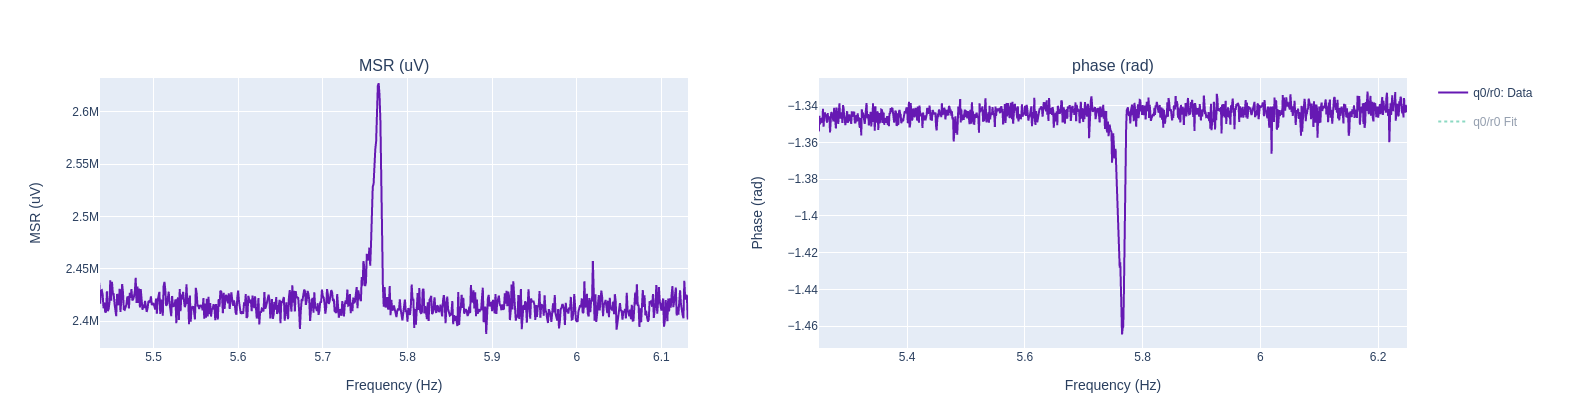
\includegraphics[width=1.3\textwidth]{characterization/figures/qubit_spec_no_relax.png}}
    \caption{Example of a qubit spectroscopy experiment with zero relaxation.}
    \label{fig:qubit_spectroscopy_no_relax}
\end{figure}

In \cref{fig:qubit_spectroscopy_no_relax} we can see the plot for a qubit spectroscopy performed without relaxation time: the physical peak is centered at $5.7$ GHz, but the apparent peak is asymmetric and shifted.

\experimentrecap
{Qubit spectroscopy}
{drive calibration}
{frequency of the qubit,\\value of $\Delta$,\\value of the coupling,\\quality factor of the qubit}
{two tone spectroscopy. First a tone is sent to the drive line, then a measurement is executed. We repeat the experiment for different frequencies for the first tone and plot the measured amplitude vs the first tone frequency. We expect to find a Lorentzian shaped peak in the opposite direction of the resonator one}